%!TEX TS-program = xelatex

\documentclass{article}

%%% This file is the preamble for the Pomona Linguistics LaTeX Paper Template, which is also used for the Quick Reference Guide. If you are brand new to writing with LaTeX, we suggest NOT messing with it, and just writing your paper using the Paper Template. If you are getting more comfortable in LaTeX and want to add packages and commands, this is where you do it (when using this template).

%For stacking text, used here in autosegmental diagrams
\usepackage{stackengine}

%To combine rows in tables
\usepackage{multirow}

%geometry helps manage margins, among other things.
\usepackage[margin=1in]{geometry}

%Gives some extra formatting options, e.g. underlining/strikeout
\usepackage{ulem}

%For putting links into papers, also helps make cross-references in the paper smart references
\usepackage[colorlinks = true,
            linkcolor = blue,
            urlcolor  = blue,
            citecolor = blue,
            anchorcolor = blue]{hyperref} %smarter cross-references, these options turn links blue

%Use package/command below to create a double-spaced document, if you want one. Uncomment BOTH the package and the command (\doublespacing) to create a doublespaced document, or leave them as is to have a single-spaced document.
%\usepackage{setspace}
%\doublespacing 

%paragraph formatting
\usepackage[parfill]{parskip}
\setlength{\parskip}{5pt} %plus 1 minus 1}
\setlength{\parindent}{30pt}
\usepackage{titlesec}

%use for special OT tableaux symbols like bomb and sad face. must be loaded early on because it doesn't play well with some other packages
\usepackage{fourier-orns}

%Basic math symbols 
\usepackage{pifont}
\usepackage{amssymb}

%%%Gives shortcuts for glossing. The use of this package is NOT explained in the Quick Reference Guide, but the documentation is on CTAN for those that are interested. MJKD finds it handy for glossing. (https://ctan.org/pkg/leipzig?lang=en)
\usepackage{leipzig}

%Tables
\usepackage{caption} %For table captions
\usepackage{booktabs} %helps format tables

%For citations and bibliography - as of 9.1.2019 we don't explain citations in this Quick Reference Guide, but Pedro Martin's tutorial does (see links in the Guide).
\usepackage{natbib}

%For OT-style tableaux
\usepackage{ot-tableau}

%Fonts
\usepackage[no-math]{fontspec} %This allows you to enter (via an IPA kayboard) IPA fonts and other symbols directly into LaTeX. Requires a particular setyp, see below.
\usepackage{libertine} %A font that actually contains many IPA symbols. This is the font you see in the preview to the right.

%to use these fonts, be sure that your typesetting engine is set to "XeLaTeX." In Overleaf, go to the Menu link on the top left (by the Overleaf icon), and under Settings be sure that the Compiler is set to "XeLaTeX." If you accessed this document via the Overleaf Pomona Linguistics template, all of this was already done for you.

%The Pomona Linguistics Paper Template in Overleaf is already set up for this, but you may run into this problem if you start building your own documents.

%highlights text with \hl{text}
\usepackage{color, soul}

%Drawing Syntax Trees
\usepackage[linguistics]{forest}

%This specifies some formatting for the forest trees to make them nicer to look at
\forestset{
  nice nodes/.style={
    for tree={
      inner sep=0pt,
      fit=band,
    },
  },
  default preamble=nice nodes,
}

%% For numbered and glossed examples %%
\usepackage{gb4e}



%Changes the \maketitle command to be smaller and take up less space on a page. 
\makeatletter         
\def\@maketitle{   % custom maketitle 
\noindent {\Large \bfseries \color{black} \@title}  \\ \hrule \noindent \@author \\ \@date  
}

%The code below will draw a circle around a piece of text. This is very useful for drawing attention to a word in a data example. use the command \circled{text} where the argument (`text' here) is what you want to be circled. This is illustrated in the Quick Reference Guide and the Paper Template.

\usepackage{tikz}

\newcommand{\circled}[1]{\begin{tikzpicture}[baseline=(word.base)]
\node[draw, rounded corners, text height=8pt, text depth=2pt, inner sep=2pt, outer sep=0pt, use as bounding box] (word) {#1};
\end{tikzpicture}
}


%%%%%%%%%%%%%%%%%%%%%%%%%%%%%%%%%%%%%%%%%%%%%%%%%%%%%%%%%%%%
%%%%%%%%%%%%%%%%%%%%%%%%%%%%%%%%%%%%%%%%%%%%%%%%%%%%%%%%%%%%

% Useful Ling Shortcuts

\RequirePackage{leipzig}
%\RequirePackage{mathtools} % for \mathrlap

% % % Shortcuts  (borrowed from JZ, I'm still unsure exactly what xspace requires)
\RequirePackage{xspace}
\xspaceaddexceptions{]\}}

%This makes the \emptyset command be a nicer one
\let\oldemptyset\emptyset
\let\emptyset\varnothing
\newcommand{\nothing}{$\emptyset$}

%Not all of these are explained in the Quick Reference Guide, but they are here bc they are relevant to some of our students.
\newcommand{\1}{\rlap{$'$}\xspace}
\newcommand{\0}{\rlap{\textsuperscript{$ˆ{\circ}$}}\xspace}
\newcommand{\Lb}[1]{$\text{[}_{\text{#1}}$ } %A more convenient left bracket
\newcommand{\Rb}[1]{$\text{]}_{\text{#1}}$ } %A more convenient left bracket
\newcommand{\gap}{\underline{\hspace{1.2em}}}
\newcommand{\vP}{\emph{v}P}
\newcommand{\lilv}{\emph{v}}
\newcommand{\Abar}{A$'$-} %A more convenient A-bar notation
\newcommand{\ph}{$\varphi$\xspace} %A more convenient phi
\newcommand{\pro}{\emph{pro}\xspace}
\newcommand{\subs}[1]{\textsubscript{#1}} %A more convenient subscript
%\newcommand{\hd}{$^{\circ}$\xspace} %Symbol for printing head / degree symbol
\newcommand{\spells}{$\Longleftrightarrow$} %spellout arrow for morph spellout rules
\newcommand{\tr}[1]{\textit{t}\textsubscript{\textit{#1}}} %easy traces with subscript
\newcommand{\supers}[1]{\textsuperscript{#1}}

% Abbreviations for glossing, based on Leipzig
\newleipzig{hab}{hab}{habitual}
\newleipzig{rem}{rem}{remote}
\newleipzig{sm}{sm}{subject marker}
\newleipzig{t}{t}{tense}
\newleipzig{aa}{aa}{anti-agreement}
\newleipzig{pron}{pron}{pronoun}
\newleipzig{rec}{rec}{recent}
\newleipzig{om}{om}{object marker}
%\newleipzig{ipfv}{ipfv}{imperfective}
\newleipzig{asp}{asp}{aspect}
\newleipzig{lk}{lk}{linker}
\newleipzig{pcl}{pcl}{particle}
\newleipzig{stat}{stat}{stative}
\newleipzig{ints}{ints}{intensive}
\newleipzig{ascl}{ascl}{assertive subject clitic}
\newleipzig{nascl}{nascl}{non-assertive subject clitic}
\newleipzig{ta}{ta}{tense and/or aspect}
\newleipzig{assoc}{assoc}{associative marker}
\newleipzig{hon}{hon}{honorific}
%\newleipzig{whprt}{wh}{\wh particle}
\newleipzig{sa}{sa}{subject agreement}
\newleipzig{conj}{conj}{conjunction}
%\newleipzig{loc}{loc}{locative}
\newleipzig{expl}{expl}{expletive}
\newleipzig{rcm}{rcm}{reciprocal marker}
\newleipzig{pers}{pers}{persistive}
%\newleipzig{}{}{} %this is just to copy for when I want to add more

%%%%%%%%%%%%%%%%%%%%%%%%%%%%%%%%%%%%%%%%%%%%%%%%%%%%%%%%%%%%
%%%%%%%%%%%%%%%%%%%%%%%%%%%%%%%%%%%%%%%%%%%%%%%%%%%%%%%%%%%%

%A couple of packages that seemed to prefer being called toward the end of the preamble

%This package provides macros for typesetting SPE-style phonological rules.
\usepackage{phonrule}

%For using Greek letters outside of math mode.
\usepackage{textgreek}


%Random, lets us use the XeLaTeX logo. Not important to the template at all.
\usepackage{metalogo}


%%%%%%%%%%%%
%% This is the end of the PREAMBLE
%%%%%%%%%%%



\title{Parallel implementation of zlib compression \& decompression}
\author{\textbf{Authors: Pengyun Zhao, Zian Ke}\\\textbf{Andrew ID: pengyunz, ziank}}

\date{\today} 

\begin{document}


\maketitle

\section{Summary}
We are going to implement a parallelized version of zlib, a library used for data compression and decompression, and benchmark its performance against the sequential version.

\section{Background}
zlib is a software library used for data compression and is an abstraction of the DEFLATE and INFLATE algorithms. It is an important library used in major programming languages and operating systems. 

\noindent The DEFLATE algorithm, used by zlib and will be our targer for parallelism, is a lossless data compression algorithm that uses a combination of two compression strategies -- Huffman coding and LZ77 compression. The algorithm first breaks data into blocks, after which LZ77 is first used for duplicate string elimination (duplicate strings are replaced with pointers) followed by applying Huffman coding for bit reduction to replace commonly used symbols with shorter representations and less commonly used symbols with longer representations. The decompression algorithm, INFLATE, is a simple reversal of the process.
\begin{figure}[!h]
\begin{center}
    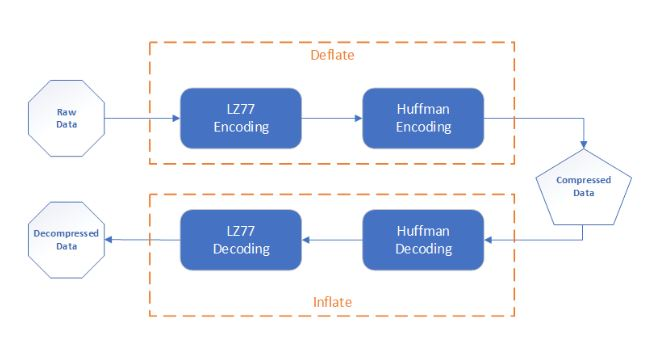
\includegraphics[height = 6cm]{Diagram.JPG}
    \caption{Diagram for the DEFLATE and INFLATE algorithm}
\end{center}
\end{figure}

\section{The Challenge}
Obviously, the zlib algorithm will have very long running time when encountering data of large scale, but we can see from the characteristic of the algorithm breaking data stream into blocks that it naturally allows for parallelism. The current bottleneck is its time spent on data I/O, duplicate search and elimination (across the whole data stream) and encoding data with Huffman coding. By distributing data chunks among processes, we may be able to achieve a great speedup of the performance.

\noindent The difficulty of parallelism lies in the dependence between consecutive chunks: the latter bytes of a deflated stream depend on the earlier bytes of that stream. A solution to this problem is to supply a certain amount of uncompressed data proceeding a particular chunk. We may also need to find a way to share the same dictionary used in encoding among multiple threads.

\section{Resources}
\begin{itemize}
    \item To have a comprehensive understanding of the zlib algorithms, we can read the article ``An Explanation of the Deflate Algorithm'' by Antaeus Feldspar and the implementation of \href{https://github.com/golang/go/tree/master/src/compress/zlib}{zlib} by the Go authors.
    \item Mark Adler, one of the authors of zlib, has completed a parallel implementation of gzip, named \href{https://zlib.net/pigz}{pigz}. This implementation will give us the basic ideas of making the DEFLATE and INFLATE algorithms parallelized.
    \item We'll also take \href{https://github.com/klauspost/pgzip}{pgzip}, a Go implementation of parallel gzip compression \& decompression, as reference, as we are going to implement the parallel zlib with Go and gzip shares similar underlying algorithms with zlib.
    \item Our benchmarks will be run on multi-core servers, such as the GHC and Latedays machines.
\end{itemize}

\section{Goals \& Deliverables}
Goals that we plan to achieve:
\begin{itemize}
    \item Implement a parallelized version of zlib in Go that produces correct compression and decompression results and is fully compatible with the standard Go zlib package, i.e.,  the data compressed by our parallel zlib can be decompressed by the standard zlib, and vice versa.
    \item Achieve noticeable speedup compared to the original sequential implementation.
    \item Have a comprehensive analysis on the implementation for different kinds of workloads. What are the new bottlenecks? What kind(s) of workload is suited for the parallel implementation?
\end{itemize}

\noindent Goals that we hope to achieve:
\begin{itemize}
    \item Achieve similar performance (or even better) with the currently released versions of parallel implementations.
    \item Prove the efficiency of parallel zlib in real-world applications such as large file compression and transport.
    \item Aim for open source release as a third-party Go package.
\end{itemize}

\noindent To ensure the correctness of our implementation, we need to write a test suite with high code coverage. We can take the unit tests of the standard Go zlib package as reference and reuse the same data as input. It's also important to write tests with large number of Goroutines and have the Go Race Detector turned on, in order to check whether any race condition exists.

\noindent To test the performance of our immplementation, we need to run benchmarks against the standard Go zlib package, and study the relationship between speedup and number of processors. The benchmarks will be run on multi-core servers, such as the GHC and Latedays machines, or cloud instances with more processors such as Amazon EC2 c5.9xlarge if necessary.

\noindent At the final poster session, we expect to present graphs of our benchmark results, as well as give a demonstration of data compression and decompression using our parallel zlib and show its compatibility with the standard zlib.

\section{Platform Choice}
The language we are going to use is Go. Go is proved to perform very well for concurrency. As the parallelized version of zlib is mainly based on multi-threading, we think Goroutine can be a powerful tool to achieve both high performance and concise implementation. We also plan to run benchmarks on our implementation against pigz, to gain more insights on the performance comparison between Go and C.

\section{Schedule}
\begin{table}[!hbp]
\begin{center}
\begin{tabular}{|c|c|}
\hline
 & Task \\ \hline
4/16-4/18 & Reviewing sequential zlib algorithms \\ \hline
4/19-4/23 & Implementation of parallel DEFLATE \\ \hline
4/24 & Checkpoint report \\ \hline
4/25-4/27 & Implementation of parallel INFLATE \\ \hline
4/28-4/30 & Correctness testing \& Debugging \\ \hline
5/1-5/2 & Datasets collection \& Benchmarks \\ \hline
5/3-5/4 & Final report \\ \hline
5/5 & Presentation \\ \hline
\end{tabular}
\end{center}
\end{table}
\end{document}

